% !TeX spellcheck = en_US
\addsection{Introduction}{\spells/magic_arrow.png}

\bigbreak

The continent of Antagarich is at war as several different Factions, led by their Heroes, battle for supremacy. Choose your Faction and Hero and banish your unruly enemies from these lands!

\hypertarget{Heroes of Might and Magic III}{\textbf{Heroes of Might and Magic III: The Board Game}} is a tactical strategy RPG board game for 1-3 players using the core box set, or more when using expansions.

\begin{multicols}{2}
\textbf{Notice}: In this rule book, game and component terms are Capitalized.
\textbf{Bold text} is used to draw attention to important rules.
\textit{Italicization} is used for gameplay examples.
\hyperlink{Heroes of Might and Magic III}{Brown colored hyperlinks} will take you to other parts of the rule book.
% The following glyphs MUST be rendered before their first use in tabular environment in all_map_locations.tex.
% Inkscape will fail otherwise.
% Other glyphs referenced over there ONLY cause no issues ¯\_(ツ)_/¯
\phantom{
  \includesvg[height=0.1px]{\svgs/artifact.svg}
  \includesvg[height=0.1px]{\svgs/spellpower.svg}
  \includesvg[height=0.1px]{\svgs/movement.svg}
  \includesvg[height=0.1px]{\svgs/2_treasure_die.svg}
}
\vfill
\columnbreak
\note{10}{Exceptions and notes with \hyperlink{Heroes of Might and Magic III}{amber colored hyperlinks} are explained in boxes like this one.
  \medskip\\
  Conflicting rule changes on components follow this priority: Player Cards, Unit Cards, Town Boards, Mission Book, this rule book.
}
\vfill
\end{multicols}

\begin{scaledfigure}[blanker]
  \centering
  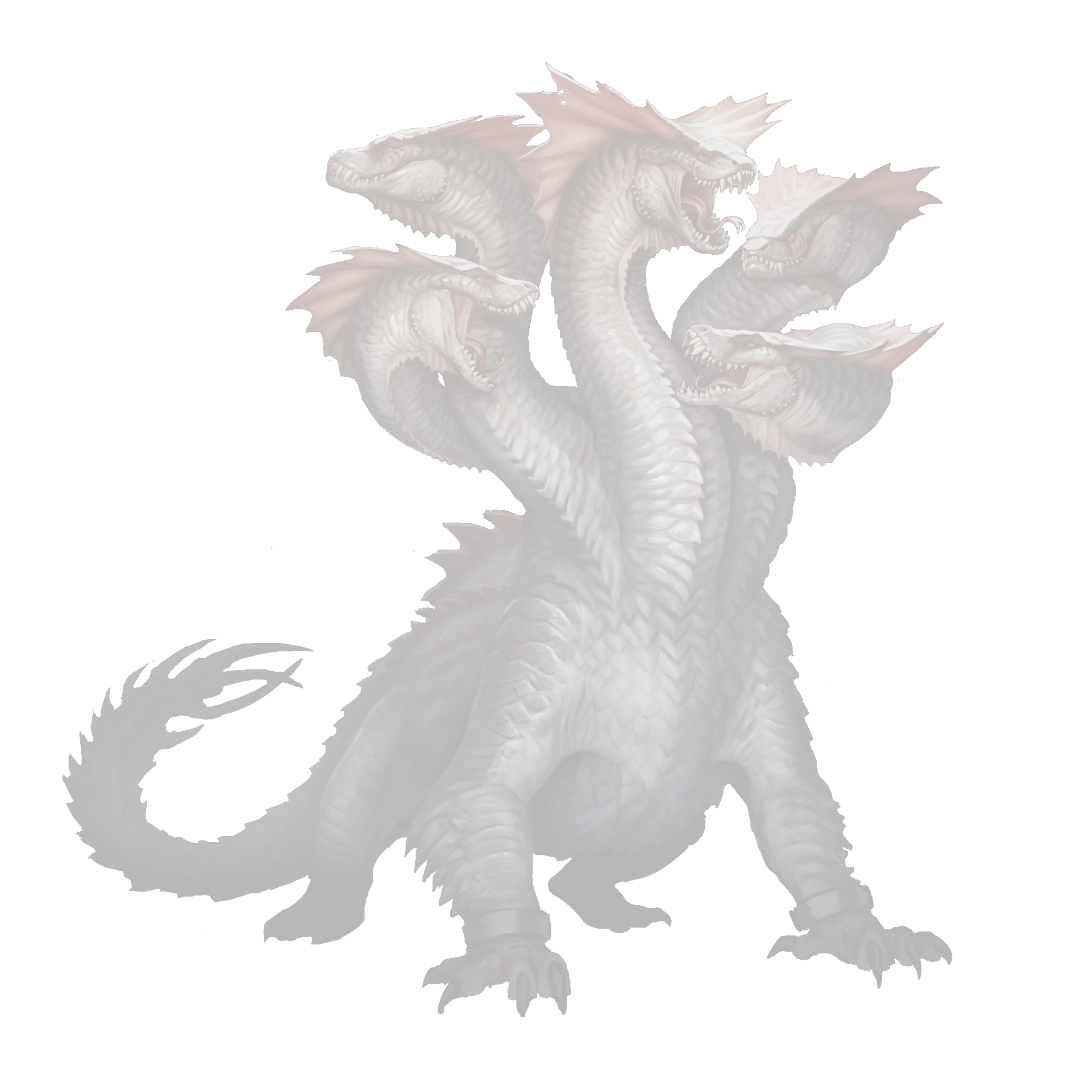
\includegraphics[width=\linewidth, height=\myspace, keepaspectratio]{\art/hydra.png}
\end{scaledfigure}
